\documentclass{beamer}
\mode<presentation>{\usetheme{IUPR}}
\usepackage[english]{babel}
\usepackage[latin1]{inputenc}
\usepackage{graphicx}
\usepackage{rotating}

\def\ra{$\rightarrow$ }
\def\rel{R}

\setbeamertemplate{navigation symbols}{}

\graphicspath{{images/}}

\definecolor{dfkiblue2}{rgb}{0.2,0.38,0.46}
\newcommand{\me}[1]{\textcolor{dfkiblue2}{#1}}
\newcommand{\ig}[2]{\includegraphics[width=#1\textwidth]{#2}}
\newcommand{\igc}[2]{\centerline{\includegraphics[width=#1\textwidth]{#2}}}

%%%%%%%%%%%%%%%%%%%%%%%%%%%%%%%%%%%%%%%%%%%%%%%%%%%%%%%%%%%%%%%%%%%%%%
\title[DCA-SS09 Lecture-2]%
{Document and Content Analysis}
\subtitle{Lecture 2 --- Document Compression} 

\author[Shafait]{Faisal Shafait}
\institute[TU-KL - IUPR - DFKI] % (optional, but mostly needed)
{
Image Understanding and Pattern Recognition\\
DFKI \& TU Kaiserslautern\\
}

\date[2009/04/28]{2009/04/28}

\AtBeginSection[]
{
   \begin{frame}
       \frametitle{Outline}
       \tableofcontents[currentsection]
   \end{frame}
}


%%%%%%%%%%%%%%%%%%%%%%%%%%%%%%%%%%%%%%%%%%%%%%%%%%%%%%%%%%%%%%%%%%%%%%
\begin{document}
%%%%%%%%%%%%%%%%%%%%%%%%%%%%%%%%%%%%%%%%%%%%%%%%%%%%%%%%%%%%%%%%%%%%%%
\begin{frame}
  \titlepage
\end{frame}
%%%%%%%%%%%%%%%%%%%%%%%%%%%%%%%%%%%%%%%%%%%%%%%%%%%%%%%%%%%%%%%%%%%%%%

\begin{frame}
  \frametitle{Motivation}
  Have you seen any files in a compressed format?
\\[6pt]

  \uncover<2->{
    zip, JPEG, MPEG, MP3, ...
\\[6pt]
}
  \uncover<3->{
   Do you know how they work?
\\[6pt]
}
  \uncover<4->{
   You should know after this lecture
}
\end{frame}




%%%%%%%%%%%%%%%% ------------------------------------ %%%%%%%%%%%%%%%%%%%%%%%


\section{Document Compression}
%\subsection{Data vs. Information}

\begin{frame}
\frametitle{Data vs. Information}
The same information can be encoded as data in many different forms,
requiring different numbers of bits, e.g.

$$0080,0090,0070,0070,0050,0010,0090,0070,0080,0090$$

\begin{itemize}
\item ASCII sequence "0080,0090,0070,0070,0050,0010,0090,0070,0080,0090"

\qquad $\Rightarrow$ 49 bytes, 392 bits

\item 32-bit integers: 80,90,70,70,50,10,90,70,80,90

\qquad $\Rightarrow$ $10\cdot 4$ bytes, 40 bytes, 320 bits

\item ASCII: "8,9,7,7,5,1,9,7,8,9" \quad $\Rightarrow$ 19 bytes, 152 bits

\item ASCII: "8977519789" \quad $\Rightarrow$ 10 bytes, 80 bits

\item ASCII-hex: 2171a14ad \quad $\Rightarrow$ 9 bytes, 72 bits

\item binary: one $34$ bit integer value \quad $\Rightarrow$ 34 bits

%\item information theoretical optimum: 22 bit sequence
% -> this statement doesn't make sense IMHO without speaking about the
% distribution, otherwise it could also be "0 bits" for this particular sequence
\end{itemize}
\end{frame}

\begin{frame}
\frametitle{Compression as Exchange of Information}
Compression can be seen as an encoding/decoding problem:
\begin{center}
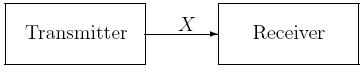
\includegraphics[width=0.8\textwidth]{communicationsystem}
\end{center}

where each side has a codebook to code or decode the message X. 

The codes can be bit-strings of arbitrary length.
Often, we require that the codes should be 
uniquely decodable by looking at one bit at a time (prefix-codes).
\end{frame}

\begin{frame}
\frametitle{Information and Coding Theory}
Consider the message $X$ of length $n$ as a random process 
with i.i.d. (independent, identically distributed) events. 
The probability for an event $i$ is $p(i)$. 

\begin{Theorem}
The \textit{information entropy} 
of a message channel, 
%which is also called \textit{amount of information} 

$$H := -\sum_i p(i)\log_2 p(i)$$

gives a lower bound on how many bits are needed to encode  
a message in the channel on the average. 
\end{Theorem}

In other words, no matter what the codebook is, a message of 
length $n$ cannot become shorter than $n\cdot H$ bits per 
symbol on the average. 

$H$ doesn't have to be integer, and if we cannot send fractional 
bits, then we cannot reach the lower bound exactly.
\end{frame}


\begin{frame}
\frametitle{Entropy as a measure of Information: Example}
The message is $0,1,0,2$. 

\begin{itemize}
\item symbols are $0,1$ and $2$ 
\item we assume $p(0)=0.5$, $p(1)=p(2)=0.25$. 
\item naive codebook: $0=\mathbf{00}$, $1=\mathbf{01}$, $2=\mathbf{10}$
\item The code is $\mathbf{00010010}$, i.e. 8 bits, or 2 bits per symbol

\item entropy: 
\begin{align*}H &= -0.5\cdot\log_2(0.5) - 0.25\cdot \log_2(0.25) - 0.25\cdot \log_2(0.25) 
\\
&= 0.5\cdot 1 + 0.25\cdot 2 + 0.25\cdot 2 = 1.5
\end{align*}

\item A better codebook would be: $0=\mathbf{0}$, $1=\mathbf{10}$, $2=\mathbf{11}$

\item The total code is $\mathbf{010011}$, requiring $6$ bits, i.e. we reach the 
theoretical bound of 1.5 bits per symbol.
\end{itemize}
\end{frame}

\begin{frame}
\frametitle{Entropy as a measure of Information: Examples}
The message $0,1,2,3,4,5,6,\dots,255$
\begin{itemize}
\item $p(i)=\frac{1}{256}$ for $i=1,\dots,256$.
\item Naive coding takes 8 bits per symbol.
\item $H = -\sum_{i=0}^{255} \frac{1}{256} \log(\frac{1}{256}) = 8$
\item So we cannot do better than naive 8-bit. 
\end{itemize}

The message $0,0,0,0,\dots$.

\begin{itemize}
\item There is only one symbol, $0$. $p(0)=1$
\item $H = 0$
\item We don't have to send anything. We agree on a codebook where "nothing" is mapped to "0". 
\item problem ?
\end{itemize}

%These calculations assume that $n$ is known. 
%For image encoding, this usually is not the case, but is has to be encoded as well. 
%The codebook either has to be sent as well, or sender and receiver agree on it implicitly, 
%e.g. by choice of the image format. 
\end{frame}



\begin{frame}
\frametitle{Variable Length Coding (VLC)}
The codes we send do not have to be of identical length:

\begin{itemize}
\item original: 128 128 128 128 128 129 129 129 129 130 131 132
\item usual 8-bit representation: $12\cdot 8 = 96$ bits

\item Entropy: 

-- $p(0,\dots,127)=0$

-- $p(128)=\frac{5}{12}=0.416$

-- $p(129)=\frac{4}{12}=0.333$

-- $p(130)=\frac{1}{12}\approx 0.083$

-- $p(131)=\frac{1}{12}\approx 0.083$

-- $p(132)=\frac{1}{12}\approx 0.083$

-- $p(133,\dots,255)=0$
\begin{align*}
H &= -\frac{5}{12}\cdot \log_2(\frac{5}{12}) - \frac{1}{3}\cdot \log_2(\frac{1}{3}) 
- 3\cdot \frac{1}{12}\cdot \log_2(\frac{1}{12}) 
\\
&\approx 1.95
\end{align*}
\end{itemize}
\end{frame}

\begin{frame}
\frametitle{Utilizing if fewer than 256 values occur}
\begin{itemize}
\item original: 128 128 128 128 128 129 129 129 129 130 131 132
\item We have 5 distinct symbols, so we can use a 3 bit code:

-- $128 \Rightarrow \mathbf{000}$

-- $129 \Rightarrow \mathbf{001}$

-- $130 \Rightarrow \mathbf{010}$

-- $131 \Rightarrow \mathbf{011}$

-- $132 \Rightarrow \mathbf{100}$

\item $3$ bits per symbol means $12\cdot 3 = 36$ bits in total
\end{itemize}
\end{frame}

\begin{frame}
\frametitle{Variable Length Coding (VLC) II}
\begin{itemize}
\item In the previous example, 132 is uniquely identified after 1 bit:

-- $128 \Rightarrow \mathbf{000}$

-- $129 \Rightarrow \mathbf{001}$

-- $130 \Rightarrow \mathbf{010}$

-- $131 \Rightarrow \mathbf{011}$

-- $132 \Rightarrow \mathbf{1}$
\item The message becomes $3+3+3+3+3+3+3+3+3+3+3+1= 34$ bits

\item Expected rate: $\frac{5}{12}\cdot 3 + \frac{4}{12}\cdot 3 + \frac{1}{12} 3 + \frac{1}{12} 3 + \frac{1}{12} \cdot 1 = 2.834$ bits per symbol
\end{itemize}
\end{frame}

\begin{frame}
\frametitle{Variable Length Coding (VLC) III}
\begin{itemize}
\item In general, it is better to code frequent symbols with short codes.
\item Since $128$ is more frequent than $132$, it is better to use 
the single $\mathbf{1}$ for 128 and the longer codes for the less frequent 
values

-- $128 \Rightarrow \mathbf{1}$

-- $129 \Rightarrow \mathbf{000}$

-- $130 \Rightarrow \mathbf{001}$

-- $131 \Rightarrow \mathbf{010}$

-- $132 \Rightarrow \mathbf{011}$

\item Expected rate: $\frac{5}{12}\cdot 1 + \frac{4}{12}\cdot 3 + \frac{1}{12} 3 + \frac{1}{12} 3 + \frac{1}{12} \cdot 3 = 2.168$ 
\item Signal length: $1+1+1+1+1+3+3+3+3+3+3+3=26$ bits
\end{itemize}
\end{frame}

\begin{frame}
\frametitle{Huffman Codes}
\begin{itemize}
\item Huffman codes can be constructed for any given distribution

-- $128 \Rightarrow \mathbf{1}$

-- $129 \Rightarrow \mathbf{01}$

-- $130 \Rightarrow \mathbf{001}$

-- $131 \Rightarrow \mathbf{0000}$

-- $132 \Rightarrow \mathbf{0001}$
         
\item Expected rate: $\frac{5}{12}\cdot 1 + \frac{4}{12}\cdot 2 + \frac{1}{12} 3 + \frac{1}{12} 4 + \frac{1}{12} \cdot 4 = 2.0$
\item Encoded signal: $\mathbf{111110101010100100000001}$ has 24 bits
%
\item Lower bound from coding theorem is $12\cdot 1.95 = 23.4$

$\Rightarrow \ 24$ is optimal. 
\end{itemize}
\end{frame}



\begin{frame}
\frametitle{Computing Huffman Codes}
\begin{itemize}
  \item compute probabilities of all symbols
  \item arrange symbols in descending order of probability
  \item construct a tree by combining two least probability nodes
  \item assign either 1 or 0 to each branch
  \item traverse the constructed tree from root node to any leaf to find the
    code for the leaf
\end{itemize}
\end{frame}



\begin{frame}
\frametitle{Huffman Codes}
\begin{itemize}
\item Huffman codes are optimal in the sense that no other code that maps
  symbols onto fixed bit-strings can create a shorter sequence.
\item It doesn't mean that they perform closely to the entropy bound, e.g. for a binary signal 
$p(0)=0.9999$, $p(1)=0.0001$: $H\approx0.0015$, but we need at least 1 bit per symbol.
\item If we drop the requirement of mapping symbols onto fixed bit-strings, we
  can do better \ra arithmetic encoding
\end{itemize}
\end{frame}

\begin{frame}
\frametitle{Signal Compression by Entropy Coding} 
\begin{itemize}
\item Storing information (text, images, sound) can be performed more 
efficiently by using a good code, based on the entropy.
\item We have achieved a compression ratio of $\frac{96}{24} = 4$ compared to 
raw 8-bit integers (PGM), just by using different symbols. 
\item Many compression utilities, e.g. WinZIP, rely on entropy codings, often by 
constructing Huffman codes.
\item Huffman compression achieves rates of approx. 2 to 3 on English text, 
and 1 to 4 on images. 
\item Huffman coding doesn't have a fixed codebook. It depends on the data.
\item In practice, the codebook and the length of the signal have to be transmitted together with the data!

%\item 1) Integrate the codebook into the data, e.g. by always
%sending a value and the code that is going to be used in future for this.
%
%\item 2) Use a fixed codebook that the sender and receiver agree on in advance
%
%\item 3) Use a code without codebook, e.g. because the values can be _calculated_ 
%from the code instead of looked up.
\end{itemize}
\end{frame}


\begin{frame}
  \frametitle{Run-Length Encoding (RLE)} In many cases, neighboring data points
  are not statistically independent, but are strongly correlated (consider
  sending a fax).

If the same values occur frequently next to each other, 
we can use \textit{Run-Length-Encoding}: 

\begin{itemize}
\item original: 0 0 0 0 0 0 1 1 1 1 1 0 0 0 0 0 1 1 0 0 0 0 0  $\Rightarrow$ 23 bit
\item $p(0)=\frac{15}{23}=0.65$, $p(1)=\frac{8}{23}=0.35$, $H\approx 0.934$
\item Run+Value: $6\times 0$, $5\times 1$, $5\times 0$, $2\times 1$, $5\times 0$
\item values alternate in fixed manner, only store run: 6 5 5 2 5
\item naive 3-bit code: 15 bits
\end{itemize}
The result can be entropy-compressed:
\begin{itemize}
\item $p(2)=\frac{1}{6}$, $p(5)=\frac{3}{5}$, $p(6)=\frac{1}{10}$ \quad $H \approx 1.23$
\item Huffman code: $5\rightarrow \mathbf{1}, 2\rightarrow\mathbf{00}, 6\rightarrow\mathbf{01}$
\item expected length: $\frac{1}{6}\cdot 2+\frac{2}{3}\cdot 1+ \frac{1}{3}\cdot 2 = 1.333$ bits per sample
\item total message: $\mathbf{0111001}$, 7 bits
\end{itemize}
%The compression ratio was improved by reducing the number of sa from 23 binary digits to 5 (small)
%integers. 
\end{frame}



\begin{frame}
\frametitle{Intermediate Summary}
\begin{itemize}
\item Information is not the same as data. The same information can be expressed (\textbf{coded}) using more or less data.
\item If we code a signal, the \textbf{entropy} of the coding alphabet is a \textbf{lower bound} on how 
many bits we will need per symbol (Shannon's Source Coding Theorem). 
\item {The lower the entropy, the more efficient we can code.}
\item {The more "peaked" the distribution, the lower its entropy.}
\item For each source, we can build a \textbf{Huffman-Code}. This is
  \textbf{optimal} (when...?).
\item The Huffman code usually does not reach the entropy bound, but it is guaranteed to stay within $1$ 
bit of it.
%\item For binary signals, Huffman Coding alone does not help anything (exercise).
\item Since entropy and coding efficiency depend on the \textbf{coding alphabet} distribution,  we can achieve better compression by first transforming a signal, e.g. by RLE.
\end{itemize}
\end{frame}


\begin{frame}
\frametitle{Making Use of Redundancy for Compression}
\small
Run-Length Encoding relies on redundancies between data samples. 
It is a general fact, that we can increase the compression ratio 
by utilizing data sample redundancy, e.g. by coding pairs of samples.

Take e.g. a pairs of data samples $(i,j)$, and use the first data sample value as a predictor 
for the second, using the relation $p(i,j) = p(j|i)p(i)$:
%
\begin{align*}
H(i,j) &= -\sum\nolimits_{i,j} p(i,j) \log_2 p(i,j)
\\
&= -\sum\nolimits_{i,j} p(j|i)p(i) \log_2 p(j|i) - \sum\nolimits_{i,j} p(j|i)p(i)\log_2 p(i)
\\
&= -\sum\nolimits_{i} p(i) \sum\nolimits_{j} p(j|i) \log_2 p(j|i) - \sum\nolimits_{i} p(i)\log_2 p(i)
\\
&= H(j|i) + H(i)
\end{align*}
\vskip -12pt
\begin{itemize}
\item A signal of length $N$ has $\frac{N}{2}$ pairs and requires at least $\frac{N}{2}\left(H(j|i)+H(i)\right)$ bits.

\item If $i$ and $j$ are independent, $p(j|i)=p(j)$ and $H(j|i)=H(j)$, and we cannot gain anything. 
\item Otherwise, $H(j|i)<H(j)$, and the theoretical bound is lower than for coding the symbols one-by-one.
\end{itemize}
\end{frame}


\begin{frame}
\frametitle{Differential Pulse Code Modulation (DPCM)}
One method to use redundancy is to use the 
previous data sample as a linear predictor and encode $s_1, s_2-s_1, s_3-s_2, \dots$. 

\begin{itemize}
\item original: 128 128 128 128 128 129 129 129 129 130 131 132
\item relative: 128 +0 +0 +0 +0 +0 +1 +0 +0 +1 +1 +1

-- $p(0)=\frac{7}{12}\approx 0.583$

-- $p(1)=\frac{4}{12}\approx 0.333$

-- $p(128)=\frac{1}{12}\approx 0.083$

\item $H = -\frac{7}{12}\cdot \log_2(\frac{7}{12}) - \frac{4}{12}\cdot \log_2(\frac{4}{12}) 
- \frac{1}{12}\cdot \log_2(\frac{1}{12}) \approx 1.28$

\item Huffman code: $0 \Rightarrow \mathbf{0}$, $1 \Rightarrow \mathbf{10}$, $128 \Rightarrow \mathbf{11}$.

\item Expected rate: $\frac{7}{12}\cdot 1 + \frac{4}{12}\cdot 2 + \frac{1}{12}\cdot 2 = 1.415$

\item Stored message: $\mathbf{11000001000101010}$, 17 bits
\end{itemize}

This method is also called \textit{Differential Pulse Code Modulation} (DPCM). 
It improves the compression ratio, if the distribution of the difference 
values has a lower entropy than the sample values themselves. 
\end{frame}

\section{Lossless Image Compression}

\begin{frame}
\frametitle{Image as Data}
An image is represented as a 2-D matrix, where each element is the intensity
value at that location in the image
\\[6pt]

All techniques studied so far can be applied to image compression as well.
\\[6pt]

\begin{itemize}
\item All methods so far are reversible processes. 
\item The result is a \textit{lossless} compression method. The decoded data is 
exactly identical to the original. 
%\item For applying DCT, this is only true mathematically. In a computer implementation, rounding 
%error will occur. 
\end{itemize}


In images we can further exploit 2-dimensional spatial correlation of data.
\end{frame}



\begin{frame}
\frametitle{Decorrelation of Image Data}
\textit{Observation:}\ A signal in which the samples are statistically 
independent cannot be coded more efficiently by combining symbols. 
\\[6pt]

In image compression one searches for representations of the image 
data such that the individual samples are \textit{uncorrelated}. The 
distribution of values should be as peaked as possible for as many 
coefficients as possible. Afterwards, applying entropy coding is very efficient. 
\\[6pt]

How can we make image data uncorrelated while keeping the 
image information?
\end{frame}

\begin{frame}
  \frametitle{Motivation for unitary transforms}
  
  \begin{itemize}
  \item Requirements of the transform:
    \begin{itemize}
    \item \textit{Energy compaction} to a small, relevant set of features \\
      for storage, transmission and analysis
    \item \textit{Decorrelation} of the image pixels
    \item \textit{Conservation of energy}
    \item \textit{Conservation of measure}, e.g. conservation of mean square differences between images 
    \item Features with small energy can be skipped (compression)
    \end{itemize}
  \item Idea:
    \begin{itemize}
    \item Represent image by weighted sum of \textit{basis images}
    \item Transform results (features) are the \textit{weighting coefficients} within the sum
    \item Basis images should be good representations of the input image
      content, so the optimal transform is image dependent
    \end{itemize}	
  \end{itemize}
\end{frame}


\begin{frame}
\frametitle{Discrete Cosine Transform (DCT)}

\begin{itemize}
\addtolength{\itemsep}{-2pt}
\item The DCT base functions do not depend on the data. 
\item They can be stored in the decoder or calculated on-the-fly.
\item We only have to transmit the coefficients.
\end{itemize}

\end{frame}



\begin{frame}
  \frametitle{2D DCT}

\begin{flushleft}
  \normalsize{The {\textcolor{blue}{2D discrete cosine transform (DCT)}} of a
    an image $S(x,y)$ is computed as:}
  \scriptsize

\[
\mathcal{S}(u,v) =
\frac{2}{N}K(u)K(v)\sum\limits_{x=0}^{N-1}\sum\limits_{y=0}^{N-1}
S(x,y)\cos\frac{(2x+1)u\pi}{2N} \cos\frac{(2y+1)v\pi}{2N}
\]
\end{flushleft}
where $K(0) = \frac{1}{\sqrt{2}}$ and $K(w) = 1$ for $w = 1,2,...,N-1$
\end{frame}



\begin{frame}
\frametitle{DCT base images}
\begin{figure}
\centering
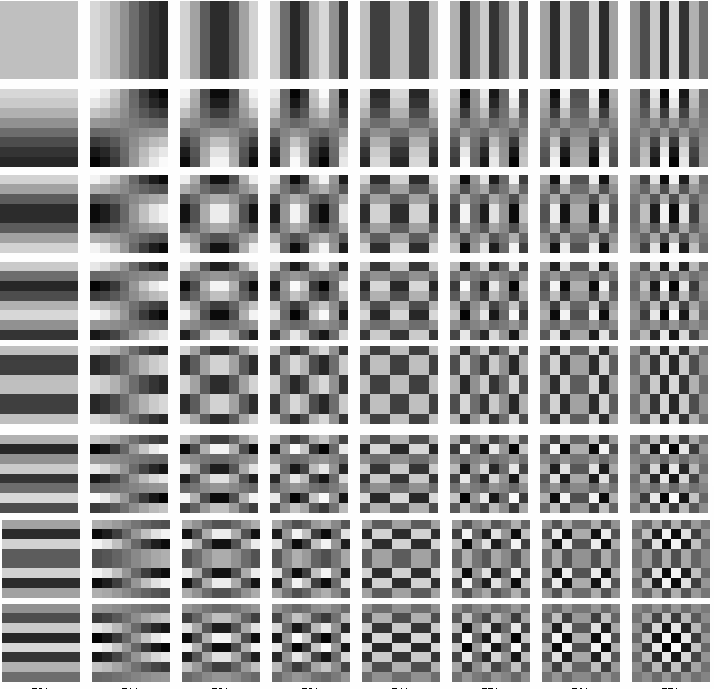
\includegraphics[width=0.47\textwidth]{dct}
\end{figure}
The DCT is a separable transform related to the FFT and can be performed in $O(n\log n)$.

\end{frame}


\begin{frame}
\frametitle{Example: 2D cosine transform of a 16x16 image}
\begin{figure}[H]
  
\includegraphics[width=  \textwidth]{Ex_BasisImages1} 
  \caption{$\frac{1}{16}S(0,0) + \frac{1}{8 \sqrt{2}}(S(0,1) + S(1,0))$}
\end{figure} 
\end{frame}

\begin{frame}
\frametitle{Example: 2D cosine transform of a 16x16 image (II)}
\begin{figure}[H]
  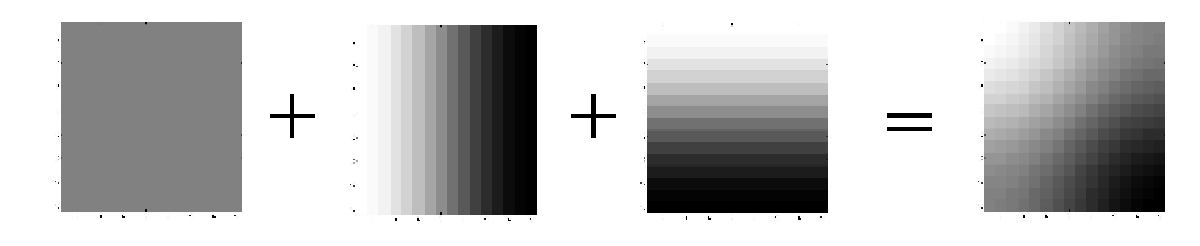
\includegraphics[width=  \textwidth]{Ex_BasisImages2} 
  \caption{$\frac{1}{16}S(0,0) + \frac{1}{8 \sqrt{2}}(S(0,1) + S(1,0))$}
\end{figure} 
\end{frame}


\begin{frame}
\frametitle{Example: 2D cosine transform of a 16x16 image (III)}
\begin{figure}[H]
  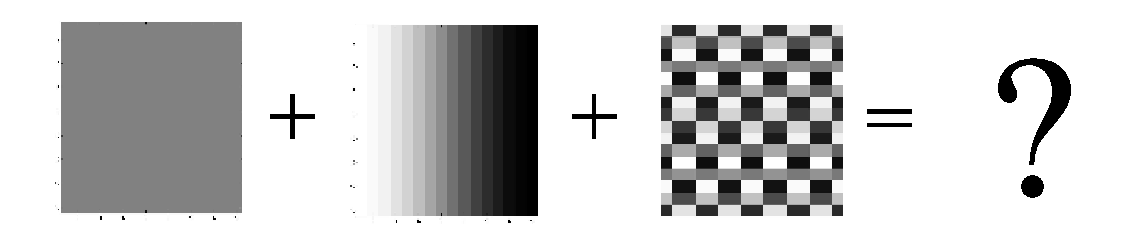
\includegraphics[width=  0.7 \textwidth]{Ex_BasisImages3} 
  \caption{$\frac{1}{16}S(0,0) + \frac{1}{8\sqrt{2}}S(0,1) + \frac{1}{8}S(6,7)$}
\end{figure} 
\end{frame}

\begin{frame}
\frametitle{Example: 2D cosine transform of a 16x16 image (IV)}
\begin{figure}[H]
  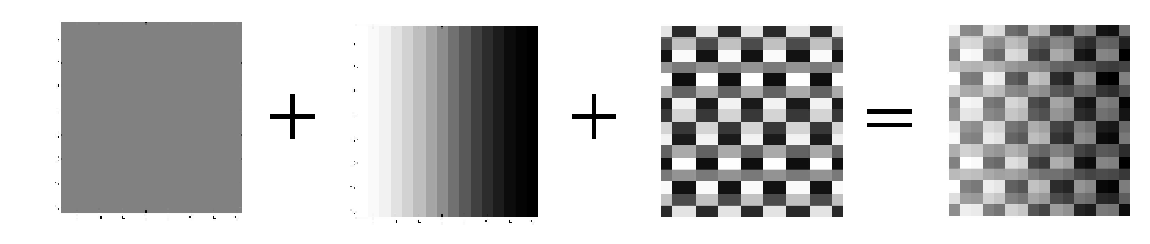
\includegraphics[width=  0.7 \textwidth]{Ex_BasisImages4} 
  \caption{$\frac{1}{16}S(0,0) + \frac{1}{8\sqrt{2}}S(0,1) + \frac{1}{8}S(6,7)$}
\end{figure} 
\end{frame}

\begin{frame}
\frametitle{Example: 2D cosine transform of a 16x16 image (V)}
\begin{figure}[H]
  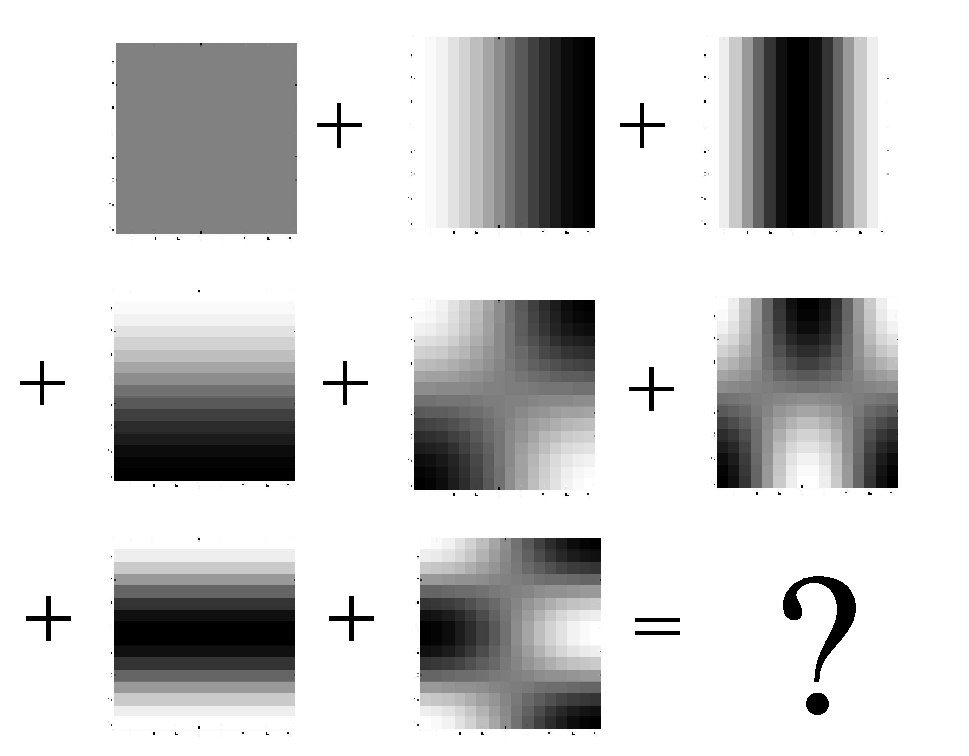
\includegraphics[width=  0.7 \textwidth]{Ex_BasisImages5} 
  \caption{$\frac{1}{16}S(0,0) + \frac{1}{8\sqrt{2}}S(0,1) + \frac{1}{8\sqrt{2}}S(1,0) + \frac{1}{8}S(1,1) + \frac{1}{8\sqrt{2}}S(2,0) + \frac{1}{8\sqrt{2}}S(0,2) + \frac{1}{8}S(2,1) + \frac{1}{8}S(1,2)$}
\end{figure} 
\end{frame}

\begin{frame}
\frametitle{Example: 2D cosine transform of a 16x16 image (VI)}
\begin{figure}[H]
  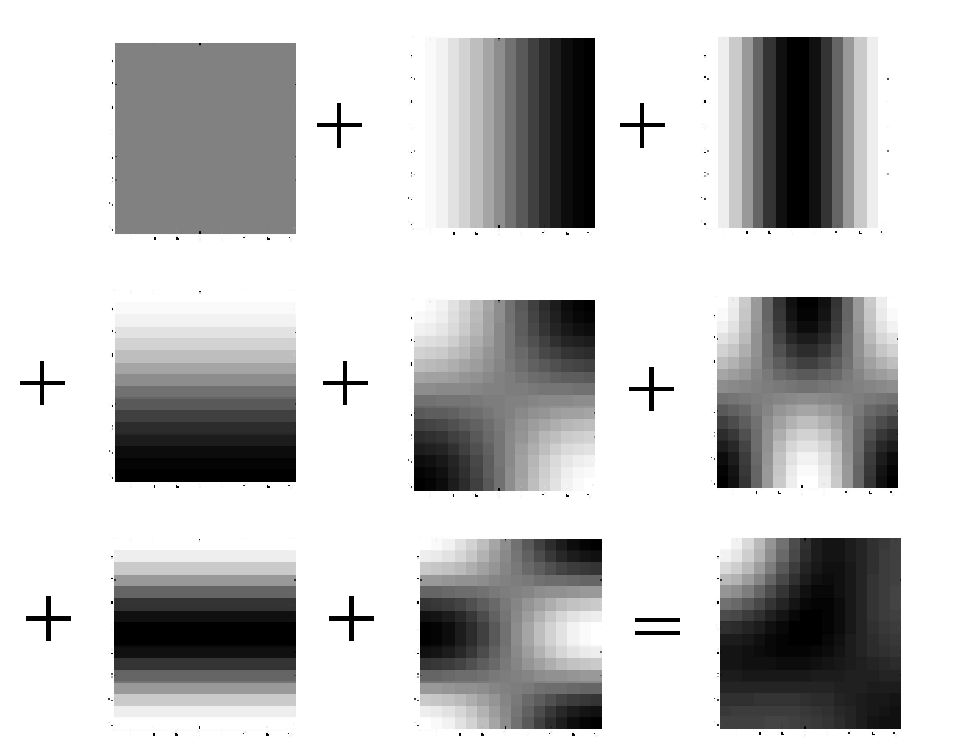
\includegraphics[width=  0.7 \textwidth]{Ex_BasisImages6} 
  \caption{$\frac{1}{16}S(0,0) + \frac{1}{8\sqrt{2}}S(0,1) + \frac{1}{8\sqrt{2}}S(1,0) + \frac{1}{8}S(1,1) + \frac{1}{8\sqrt{2}}S(2,0) + \frac{1}{8\sqrt{2}}S(0,2) + \frac{1}{8}S(2,1) + \frac{1}{8}S(1,2)$}
\end{figure} 
\end{frame}




\begin{frame}
\frametitle{Simple Methods for Image Compression}
With our knowledge so far, we can create simple methods for the compression 
of different kinds of images:\\[12pt]

For binary images: 
\begin{itemize}
\item Express the image by Run-Length-Encoding.
\item Perform entropy coding of the run values. 
\end{itemize}
This method is similar to the compression used for {TIFF} images and in {fax machines}.
\\[12pt]

For artificial images (e.g. computer graphics, screenshots)
\begin{itemize}
\item Create a predicted representation of the image data
\item Perform entropy coding of the result.
\end{itemize}
This method is similar to the \textbf{PNG} format. PNG prediction is done vertically,
each row being predicted by previous rows. In \textbf{lossless JPEG}, a pixel is 
predicted from its top, left and top-left neighbor.
\end{frame}

\begin{frame}
\frametitle{Simple Methods for Image Compression}
For natural images: 
\begin{itemize}
\item Convert RGB input to YCbCr color space. The separate brightness and color channels in YCbCr 
are less correlated.
\item Split the image (each color channel) into blocks of size $8\times 8$. 
\item For each block, calculate the 2D-DCT coefficients.
\item Arrange the coefficients into a $1D$-order (usually zig-zag).
%\item Perform prediction of the DCT coefficients by subtracting the previous (left or top) $N\times N$ block.
\item Perform entropy coding to the resulting coefficients. 
\end{itemize}

This method achieves compression ratios close to $2$. The structure is similar 
to JPEG encoding, but some crucial steps are missing. \\[6pt]

Larger blocks than $8\times 8$ improve the compression ratio but require more computing 
time and memory (DCT is $O(n\log n))$. \\[6pt]

Instead of DCT, other transforms can be used as well, e.g. wavelets. Then usually the whole 
image is treated as a single block.
\end{frame}


\section{Lossy Image Compression}

\begin{frame}
\frametitle{Lossless vs. Lossy Compression}

\begin{itemize}
\item Lossless compression relied on the removal of redundancy. % is \textit{coding} and \textit{pixel values}.
\item Lossy compression can use another powerful source of redundancy: the human
  visual system!
\item We do not only reduce the amount of data, but we discard a part of the
  information, that does not change the human perception much.
\end{itemize}
\end{frame}


\begin{frame}
\frametitle{The human visual system: Least Noticable Differences}

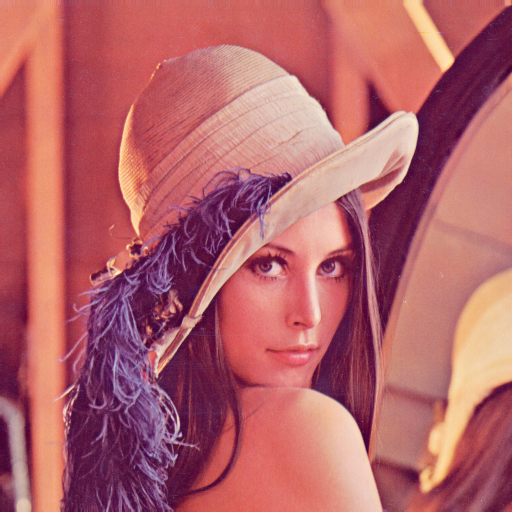
\includegraphics[width=0.47\textwidth]{lena}\ 
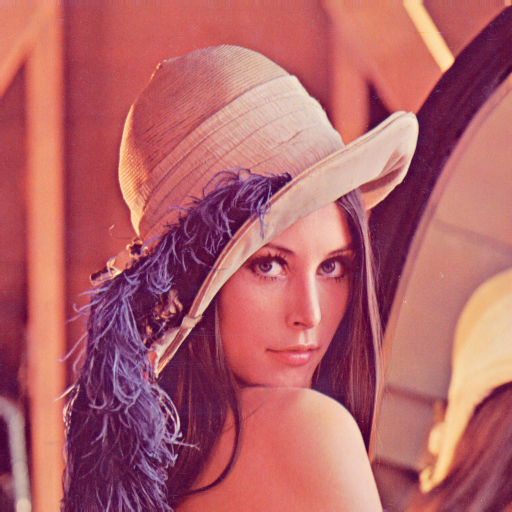
\includegraphics[width=0.47\textwidth]{lena-2}

The color depth was reduced from 8 to 7 bits per pixel per channel: 14\% size reduction
\end{frame}

\begin{frame}
\frametitle{The human visual system: High Frequencies}

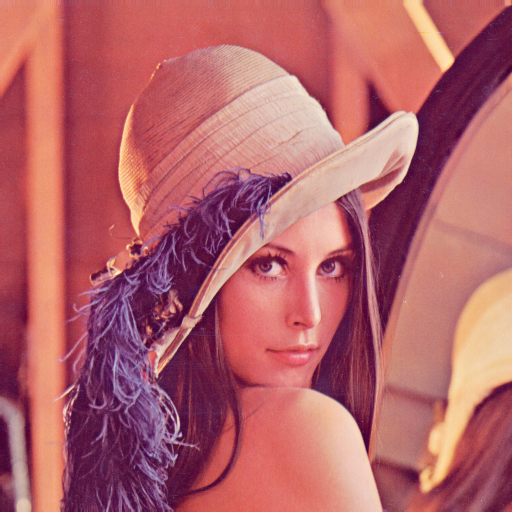
\includegraphics[width=0.47\textwidth]{lena}\ 
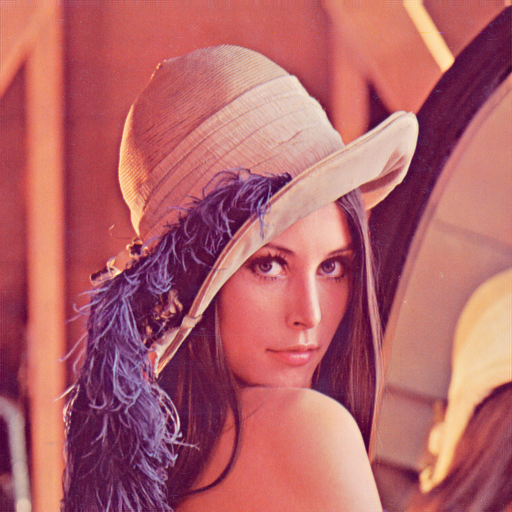
\includegraphics[width=0.47\textwidth]{lena-lowpass}

The highest frequencies were removed from the FFT spectrum: 10\% size reduction
\end{frame}


\begin{frame}
\frametitle{The human visual system: Color Resolution}

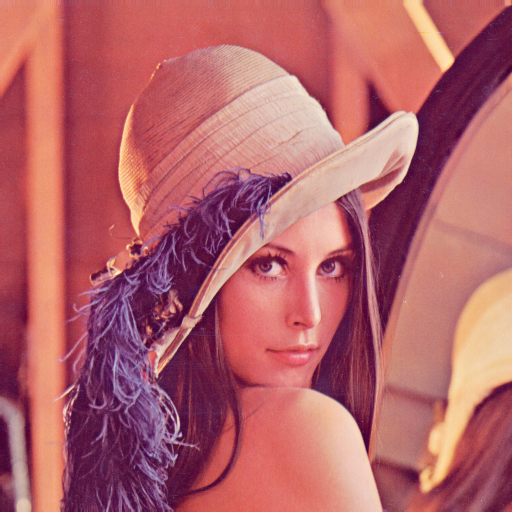
\includegraphics[width=0.47\textwidth]{lena}\ 
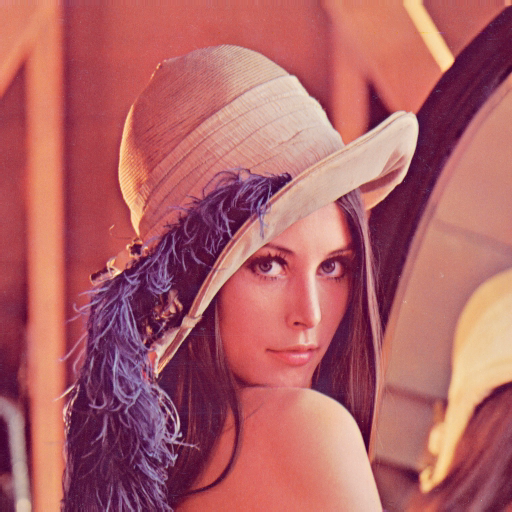
\includegraphics[width=0.47\textwidth]{lena-420}

The color channels in YCbCr were subsampled to half resolution: 50\% size reduction
\end{frame}


\begin{frame}
\frametitle{The human visual system: Resolution}

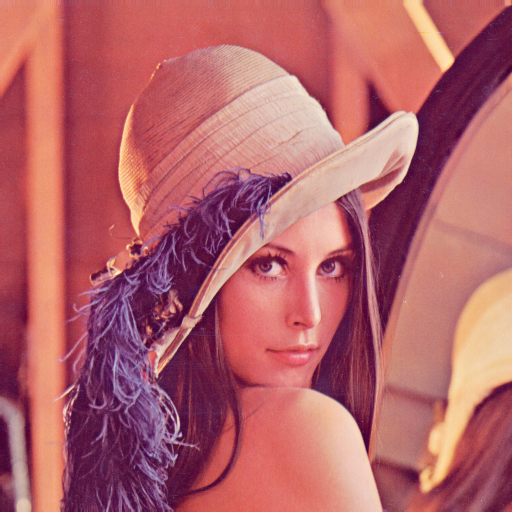
\includegraphics[width=0.47\textwidth]{lena}\ 
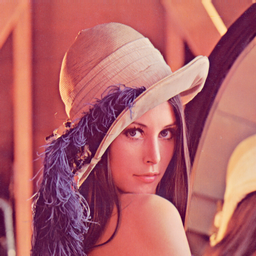
\includegraphics[width=0.47\textwidth]{lena-small}

The image was resized to 50\% resolution: 

75\% size reduction.

\end{frame}



\begin{frame}
\frametitle{JPEG compression}
JPEG compression uses all the concepts we have seen:

\begin{itemize}
\item Conversion to YCbCr color space and reduction of resolution in the color components
\item Blockwise 2D-DCT in each channel
\item Quantization of the resulting DCT coefficients
\item Predictive Encoding for the 1st quantized coefficent (DC)
\item Run-Level Encoding for the other quantized coefficients
\item Huffman Encoding of what is left
\end{itemize}
\end{frame}


\begin{frame}
\frametitle{2D-DCT of $8 \times 8$ blocks}
Luminance and Chrominance are arranged into $8\times 8$ blocks. 
A value of $128$ is subtracted from each entry and the resulting 
$8\times 8$ block is transformed using the 2D-DCT. This yields 
an $8\times 8$ block of coefficients. 
\begin{center}
%\includegraphics[width=0.2\textwidth]{image-block}$\quad\rightarrow\quad$
%\includegraphics[width=0.45\textwidth]{DCT-block}
%\includegraphics[width=0.7\textwidth]{example-DCTzigzag}

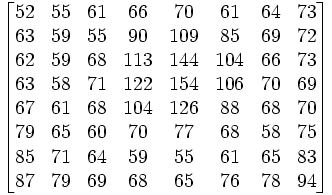
\includegraphics[height=0.22\textwidth]{image-matrix}$\rightarrow$
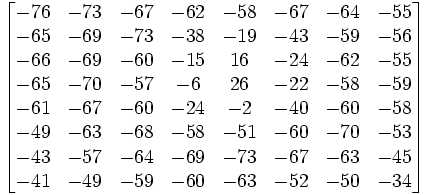
\includegraphics[height=0.22\textwidth]{subtracted-matrix}\\[6pt]
$\rightarrow$ 
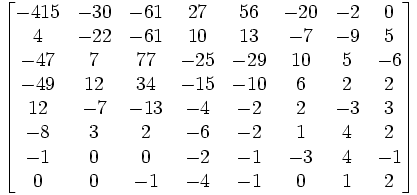
\includegraphics[height=0.22\textwidth]{DCT-matrix}
\end{center}

The $(0,0)$ (top-left) entry is called $DC$-coefficient, the other entries are called $AC$-coefficients.

\end{frame}



\begin{frame}
\frametitle{Quantization of DCT-coefficients}
The DCT coefficients are \textit{quantized} by dividing them 
by a constant and rounding to the next integer. 
Each position in the block can have a different value (\textit{quantizer}) 
to be divided by. The quantizers form quantization 
matrices for luma and chroma.
\begin{center}
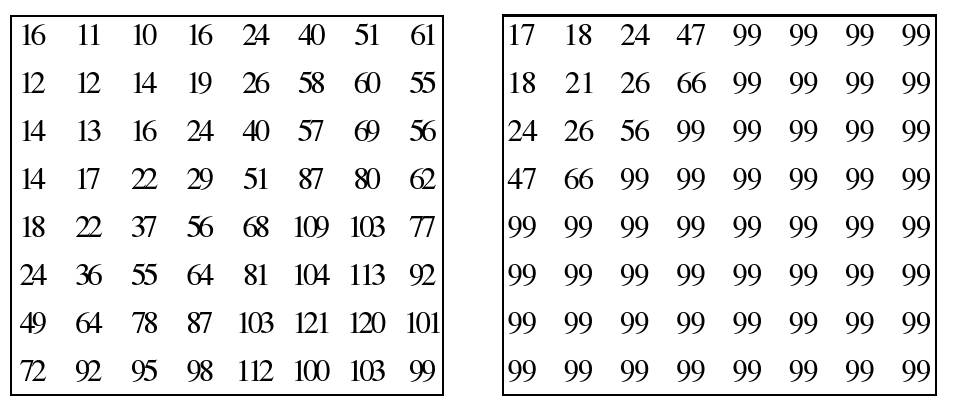
\includegraphics[height=0.26\textwidth]{quantization-matrix}
\end{center}

Quantizers are chosen with regards to the human visual system.

\begin{center}
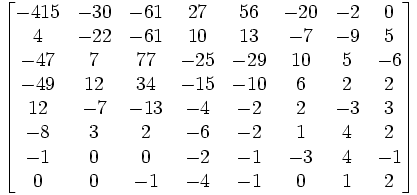
\includegraphics[height=0.2\textwidth]{DCT-matrix}\quad$\rightarrow$\quad
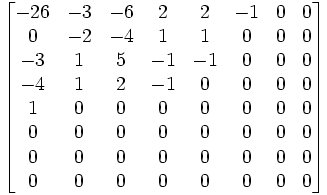
\includegraphics[height=0.2\textwidth]{quantized-matrix}
\end{center}

\end{frame}



\begin{frame}
\frametitle{Zigzag ordering}
The 2D-block entries are read out in a zigzag order

\begin{center}
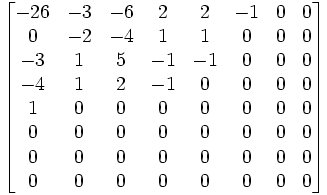
\includegraphics[height=0.25\textwidth]{quantized-matrix}\quad
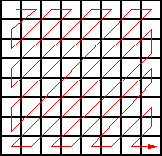
\includegraphics[height=0.25\textwidth]{zigzag}
\end{center}
%
This yields a 1D-array of size $64$:
%

-26, -3, 0, -3, -2, -6, 2, -4, 1, -4, 1, 1, 5, 1, 2, -1, 1, -1,
2, 0, 0, 0, 0, 0, -1, -1, 0, 0, 0, 0, 0, 0, 0, 0, 0, 0, 0, 0, 0, 0, 0, 0,
0, 0, 0, 0, 0, 0, 0, 0, 0, 0, 0, 0, 0, 0, 0, 0, 0, 0, 0, 0, 0, 0


\end{frame}

\begin{frame}
\frametitle{Run-Level Encoding}
The DC coefficient is predicted from the previously processed block.

\begin{center}
-26 $\mapsto$ +2
\end{center}

The AC coefficients are Run-Length encoded using $(\mathit{run},\mathit{level})$ codes.
$\mathit{run}$ is the number of zeros and $\mathit{level}$ is the following  
coefficient value. There is a special code $EOB$ for $\mathit{end\ of\ block}$.\\[12pt]

-3, 0, -3, -2, -6, 2, -4, 1, -4, 1, 1, 5, 1, 2, -1, 1, -1, 2, 0, 0, 0, 0, 0, 

-1, -1, 0, 0, 0, 0, 0, 0, 0, 0, 0, 0, 0, 0, 0, 0, 0, 0, 0, 0, 0, 0, 0, 0, 0, 

0, 0, 0, 0, 0, 0, 0, 0, 0, 0, 0, 0, 0, 0, 0\\[6pt]

becomes\\[6pt]

$(0,-3), (1,-3), (0,-2), (0,-6), (0,2), (0,-4), (0,1), (0,-4), (0,1), $

$(0,1), (0,5), (0,1), (0,2), (0,-1), (0,1), (0,-1), (0,2), (5,-1), $

$(0,-1), EOB$

\end{frame}




\begin{frame}
\frametitle{Huffman Encoding}
The Run-Level pairs are entropy encoded. The codebooks are not stored in the bitstream,
but generated by a subroutine.

\begin{itemize}
\item For DC, larger absolute values have longer codewords.

\item For AC, the codebook is specially designed for JPEG. 
\end{itemize}
\begin{center}
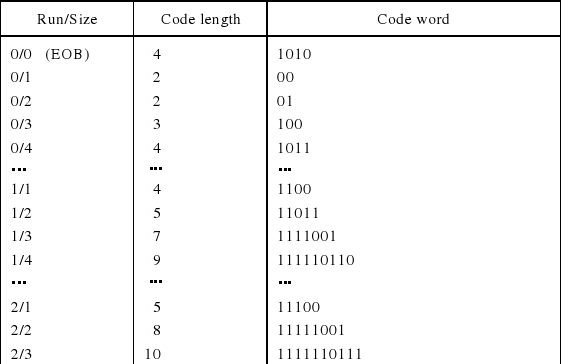
\includegraphics[height=.5\textwidth]{codes.png}
\end{center}
\end{frame}


\begin{frame}
\frametitle{JPEG decompression}
JPEG decompression applies all encoding steps in backwards order:

\begin{itemize}
\item Decoding of Huffman Codes
\item Conversion of Run-Level Codes to 1D array
\item Addition of prediction to DC coefficient
\item Dequantization of all coefficients 

$\mathit{coeff}[i] \quad\mapsto\quad \mathit{q}[i]\cdot \mathit{coeff}[i]$ 

\item Arrangement of coefficients into $8\times 8$ block
\item Inverse 2D-DCT of each block
\item Conversion to $4$ luma and $2$ chroma block to $4$ RGB blocks.
\end{itemize}

{The JPEG-standard only describes the decompression process!} 
How exactly to come up with a valid bitstream is up to the compression
software. (What are advantages of this approach?)
\end{frame}

\begin{frame}
\frametitle{Results}
%\begin{center}
\hspace*{-9mm}
\begin{tabular}{ccc}
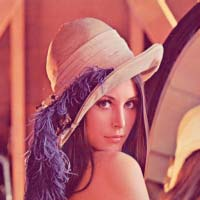
\includegraphics[height=.31\textwidth]{lena-orig}&
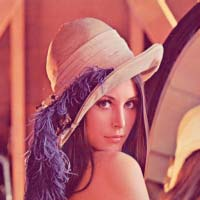
\includegraphics[height=.31\textwidth]{lena-orig}&
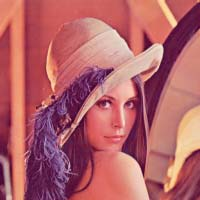
\includegraphics[height=.31\textwidth]{lena-1600}
\\[-4pt]
\scriptsize original 24 bpp, 1:1 &\scriptsize  PNG: 14.7 bpp &\scriptsize  JPEG: 1.6 bpp, 1:15 
\\[5pt]
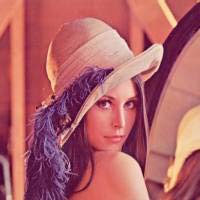
\includegraphics[height=.31\textwidth]{lena-0267}&
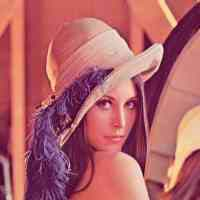
\includegraphics[height=.31\textwidth]{lena-0114}&
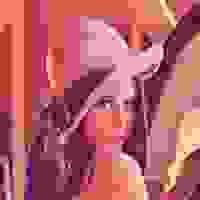
\includegraphics[height=.31\textwidth]{lena-0080}
\\[-4pt]
\scriptsize JPEG: 0.267 bpp, 1:90 &\scriptsize  JPEG: 0.114 bpp, 1:210 &\scriptsize  JPEG: 0.08 bpp, 1:300
\end{tabular}
%\end{center}
\\[3pt]

JPEG achieves good visual results, often down to 0.1 bits per pixel.
\end{frame}


\begin{frame}
\frametitle{Measuring Lossy Compression Performance}
Lossy image compression methods are measured in a rate-distortion curve:
\begin{itemize}
\item By the choice of the quantizer matrix, we can reach virtually 
any compression ratio, but at the same time, more and more image information 
is discarded. 
\item To measure the image degradation, we use the mean square error (MSE) 
or the Peak-Signal-to-Noise-Ratio (PSNR):
\begin{align*}
MSE(I_{compr},I_{orig}) &= \frac{1}{N\cdot M}{\sum_{x,y} (I_{compr}(x,y)-I_{orig}(x,y))^2}
\\
PSNR(I_{compr},I_{orig}) &= 10\cdot\log_{10} \frac{255^2}{MSE(I_{comp},I_{orig})}
\end{align*}
\item The PSNR depends strongly on the input image. 
\end{itemize}
\end{frame}


\begin{frame}{Problems of PSNR}
\begin{itemize}
\item The PSNR is only meaningful when comparing exactly the same image information.
\item It is an \textit{objective} measure, based on signal processing theory. 
\item The human visual impression is \textit{subjective}: 

-- Different people judge the image quality differently. 

-- Higher PSNR does not automatically mean better visual quality (even for the same person and the same image)

\item Many other measures have been proposed, which should reflect the subjective quality better, 
but there is no established standard. 

\item When real subjective testing is crucial, human testing is necessary. 
Usually judging images on a \textit{MOS (mean-opinion-score) scale}: 
\end{itemize}
\begin{center}
5 = \textit{excellent}, 
4 = \textit{good}, 
3 = \textit{fair}, 
2 = \textit{poor}, 
1 = \textit{bad}
\end{center}
\end{frame}

%%%%%%%%%%%%%%%%%%%%%%%%%%%%%%%%%%%%%%%%%%%%%%%%%%%%%%%%%%%%%%%%%%%%%%
\section{Compression of Textual Images}

%%%%%%%%%%%%%%%%%%%%%%%%%%%%%%%%%%%%%%%%%%%%%%%%%%%%%%%%%%%%%%%%%%%%%%%
%\begin{frame}
%  \frametitle{}
%
%Fax, JBIG, DJVU
%
%Compression of Textual Images   
%compare token-based a la djvu with Tiff/PNG    
% Concrete Examples
%
%%DatKomp04-05/Vukadinovic/ausarbeitung_vorlage/ausarbeitung_vorlage.pdf
%%http://www.leptonica.com/jbig2.html
%
%\end{frame}

%%%%%%%%%%%%%%%%%%%%%%%%%%%%%%%%%%%%%%%%%%%%%%%%%%%%%%%%%%%%%%%%%%%%%%
\begin{frame}
  \frametitle{Document Image Properties}

properties of document images (or textual images) \\ relevant for compression:
\begin{itemize}
\item binary images / high contrast
\item repetition of {\em symbols}
\item regular distribution of symbols / symbol distances
\end{itemize}


\end{frame}

%%%%%%%%%%%%%%%%%%%%%%%%%%%%%%%%%%%%%%%%%%%%%%%%%%%%%%%%%%%%%%%%%%%%%%
\begin{frame}
  \frametitle{Example Image}

\igc{0.99}{nederl}

\end{frame}

%%%%%%%%%%%%%%%%%%%%%%%%%%%%%%%%%%%%%%%%%%%%%%%%%%%%%%%%%%%%%%%%%%%%%%
\begin{frame}
  \frametitle{Compression Approaches}

approaches for compression
  \begin{itemize}
  \item standard-approaches like PNG/GIF (runs, repetitions)
  \item OCR and only save text and position 
  \item fax compression (also used in TIFF, runs, similar lines)
  \item context-dependent arithmetic coding (JBIG)
  \item token-based compression and mixed raster format (DJVU)
  \end{itemize}

JBIG=Joint Bi-level Image Experts Group\\
JPEG=Joint Photographic Experts Group

\end{frame}

%%%%%%%%%%%%%%%%%%%%%%%%%%%%%%%%%%%%%%%%%%%%%%%%%%%%%%%%%%%%%%%%%%%%%%
\begin{frame}
  \frametitle{Fax Compression}

CCITT-G3 
\begin{itemize}
\item current fax standard
\item each line encoded separately (recover from errors)
\item use Huffman coding for runs of pixels
\end{itemize}

\igc{0.4}{ccitt1}

CCITT-G4
\begin{itemize}
\item used in TIFF-G4 compression
\item lines can be encoded as in G3, or reference the previous line 
\item uses relative position of positions of color change
\end{itemize}

\igc{0.6}{ccitt3}


\end{frame}


%%%%%%%%%%%%%%%%%%%%%%%%%%%%%%%%%%%%%%%%%%%%%%%%%%%%%%%%%%%%%%%%%%%%%%
\begin{frame}
  \frametitle{Fax Compression}

\centerline{
\ig{0.7}{rle}
}

\centerline{
\ig{0.9}{fig8-14}
}


\end{frame}


%%%%%%%%%%%%%%%%%%%%%%%%%%%%%%%%%%%%%%%%%%%%%%%%%%%%%%%%%%%%%%%%%%%%%%
\begin{frame}
  \frametitle{Context-Dependent Compression}


\igc{0.25}{context1}

\igc{0.7}{contexts}

\begin{itemize}
\item context allows a much better prediction of a pixel value
\item context models have lower entropy and better compression
\end{itemize}
Example: JBIG (JBIG1)

\end{frame}


%%%%%%%%%%%%%%%%%%%%%%%%%%%%%%%%%%%%%%%%%%%%%%%%%%%%%%%%%%%%%%%%%%%%%%
\begin{frame}
  \frametitle{Token-based Compression}

  \begin{itemize}
  \item find all symbols (or tokens) \ra connected components
  \item construct a library of symbols (use repetition/similarity)
  \item compress library, sequence of symbols, and distances
  \item (lossless: compress difference image)
  \end{itemize}

Example: JBIG2

\end{frame}

%%%%%%%%%%%%%%%%%%%%%%%%%%%%%%%%%%%%%%%%%%%%%%%%%%%%%%%%%%%%%%%%%%%%%%
\begin{frame}
  \frametitle{Token-based Compression}

Construction of the library:
  \begin{itemize}
  \item for each token check if a {\em similar} token exists in the library,
   otherwise add it to the library
  \item needs a definition of similarity \ra character recognition
  \end{itemize}

Example of (dis-)similarity:
\begin{itemize}
\item perform rough pre-selection (e.g.\ by size)
\item normalize tokens with respect to center of mass
\item one of 
  \begin{itemize}
  \item weighted pixel-wise XOR
  \item Fourier coefficients
  \item flexible image matching
  \end{itemize}
\end{itemize}


\end{frame}


%%%%%%%%%%%%%%%%%%%%%%%%%%%%%%%%%%%%%%%%%%%%%%%%%%%%%%%%%%%%%%%%%%%%%%
\begin{frame}
  \frametitle{Dissimilarity of Tokens}

\igc{0.9}{templa}

\end{frame}

%%%%%%%%%%%%%%%%%%%%%%%%%%%%%%%%%%%%%%%%%%%%%%%%%%%%%%%%%%%%%%%%%%%%%%
\begin{frame}
  \frametitle{Library and Symbol Sequence}

\igc{0.99}{bib}

\footnotesize
\begin{tabular}{l l}
\begin{tabular}{|r|r|r|r|}
\hline \multicolumn{4}{|c|}{Symbols and Distances} \\ 
\hline $\Delta x$ & $\Delta y$  & No.& Symbol \\
\hline 
19& 62  & 1 &---   \\
24& 7   & 2 &  R   \\
2 & -1  & 3 &  e   \\
3 & 0   & 4 &  s   \\
4 & 0   & 5 &  o   \\
2 & -1  & 6 &  l   \\
3 & 0   & 7 &  u   \\
3 & 0   & 8 &  t   \\
3 & 0   & 9 & \i   \\
-8& -25 & 10&  .   \\
7 & 25  & 3 &  e   \\
15& 0   & 11&  v   \\
 \hline
\end{tabular} &
\ig{0.55}{bsp}
\end{tabular}


\end{frame}

%%%%%%%%%%%%%%%%%%%%%%%%%%%%%%%%%%%%%%%%%%%%%%%%%%%%%%%%%%%%%%%%%%%%%%
\begin{frame}
  \frametitle{Mixed Raster Compression (MRC)}

example: DJVU (also: JBIG2)

\vfill
split image into layers and encode separately with appropriate method
    \begin{itemize}
    \item text layer \ra token-based at about 300-400dpi
    \item text-color layer (usually black) \ra image at about 25dpi
    \item background, images, texture \ra image at about 100dpi
    \end{itemize}

\end{frame}


%%%%%%%%%%%%%%%%%%%%%%%%%%%%%%%%%%%%%%%%%%%%%%%%%%%%%%%%%%%%%%%%%%%%%%
\begin{frame}%[fragile]
  \frametitle{Mixed Raster Compression (MRC)}
\rule{-1em}{0pt}%
\begin{tabular}{cc}
  \ig{0.45}{djv1} & 
  \begin{minipage}[b]{0.6\textwidth}
  \centering
  \ig{0.48}{djv2}~~\ig{0.48}{djv4}\\[0.5ex]
  \ig{0.48}{djv3}
  \end{minipage}
\end{tabular}

\end{frame}


%%%%%%%%%%%%%%%%%%%%%%%%%%%%%%%%%%%%%%%%%%%%%%%%%%%%%%%%%%%%%%%%%%%%%%
\begin{frame}
\frametitle{Summary of Image Compression}
\begin{itemize}
\item Compression uses (different forms of) \textbf{redundancy}
\end{itemize}
\begin{itemize}
\item \textbf{Lossless compression} reduces data without losing information: entropy coding (Huffman) and run-level encoding.
\item Symbols are better compressible if their distribution is strongly peaked.
\item Pixel correlations can be used to make probability distributions more peaked: direct prediction or PCA/DCT/DWT
\end{itemize}
\begin{itemize}
\item \textbf{Lossy compression} achieves much higher compression ratios by discarding information.
\item Properties of the human visual system are used to only remove "invisible" information:

-- Greyscale values or DCT coefficients are quantized.

-- High frequencies quantized stronger than low frequencies.

-- Color information is downscaled compared to brightness.

\end{itemize}
\end{frame}

\begin{frame}
\frametitle{Audio Compression}
How would you design an audio compression system (MP3)?
\end{frame}


%%%%%%%%%%%%%%%%%%%%%%%%%%%%%%%%%%%%%%%%%%%%%%%%%%%%%%%%%%%%%%%%%%%%%%
%%%%%%%%%%%%%%%%%%%%%%%%%%%%%%%%%%%%%%%%%%%%%%%%%%%%%%%%%%%%%%%%%%%%%%
%%%%%%%%%%%%%%%%%%%%%%%%%%%%%%%%%%%%%%%%%%%%%%%%%%%%%%%%%%%%%%%%%%%%%%
\end{document}
%%%%%%%%%%%%%%%%%%%%%%%%%%%%%%%%%%%%%%%%%%%%%%%%%%%%%%%%%%%%%%%%%%%%%%
%%%%%%%%%%%%%%%%%%%%%%%%%%%%%%%%%%%%%%%%%%%%%%%%%%%%%%%%%%%%%%%%%%%%%%
%%%%%%%%%%%%%%%%%%%%%%%%%%%%%%%%%%%%%%%%%%%%%%%%%%%%%%%%%%%%%%%%%%%%%%



%%%%%%%%%%%%%%%%%%%%%%%%%%%%%%%%%%%%%%%%%%%%%%%%%%%%%%%%%%%%%%%%%%%%%%
\section{}

%%%%%%%%%%%%%%%%%%%%%%%%%%%%%%%%%%%%%%%%%%%%%%%%%%%%%%%%%%%%%%%%%%%%%%
\subsection{}

%%%%%%%%%%%%%%%%%%%%%%%%%%%%%%%%%%%%%%%%%%%%%%%%%%%%%%%%%%%%%%%%%%%%%%
\begin{frame}
  \frametitle{}

\end{frame}


%%%%%%%%%%%%%%%%%%%%%%%%%%%%%%%%%%%%%%%%%%%%%%%%%%%%%%%%%%%%%%%%%%%%%%
\section{}

%%%%%%%%%%%%%%%%%%%%%%%%%%%%%%%%%%%%%%%%%%%%%%%%%%%%%%%%%%%%%%%%%%%%%%
\begin{frame}
  \frametitle{}

\end{frame}


